% This is a sample LaTeX input file.  (Version of 12 August 2004.)
%
% A '%' character causes TeX to ignore all remaining text on the line,
% and is used for comments like this one.

\documentclass{article}      % Specifies the document class

\usepackage{graphicx}		 % Need this to include images
\usepackage{hyperref}
\usepackage{amsmath}
\usepackage{amsthm}
\usepackage{xcolor}

%% Define a HUGE 
\makeatletter
\newcommand\HUGE{\@setfontsize\Huge{50}{60}}
\newcommand\todo[1]{\textcolor{blue}{#1}}
\makeatother

\newtheorem{theorem}{Theorem}[section]
\newtheorem{invariant}{Invariant}
\newtheorem{lemma}{Lemma}[section]
\newtheorem{example}{Example}[subsection]

\DeclareMathOperator\mate{mate}

\begin{document}             % End of preamble and beginning of text.

 
%titlepage
\thispagestyle{empty}
\begin{center}
\begin{minipage}{0.9\linewidth}
\flushright
	      		 
	%University logo
    
\includegraphics[width=0.5\linewidth]{univie.jpg}\par
    \vspace{1.5cm}
\centering 	
    % Title
	{\scshape{\HUGE Bachelorarbeit\par}}
	\vspace{1cm}
	%Thesis title
    {\scshape{\Large engineering algorithms for dynamic maximal matchinga\par}}
    \vspace{2cm}
    
  
 Verfasser  \linebreak
 {\Large Richard Paul\par}
 	\vspace{1.5cm}
angestrebter akademischer Grad\linebreak
 {\Large Bachelor of Science (BSc)\par}
	\vspace{1.5cm}

\flushleft
	

\begin{tabular}{ll}
Wien, 2018 \linebreak
\vspace{1cm}&   \\
  Studienkennzahl lt. Studienblatt: & A 033 521 \vspace{0.3cm} \\ 
  Fachrichtung: & Informatik  -  Scientific Computing \vspace{0.3cm} \\
  Betreuer: & Dr. rer. nat. Christian Schulz  \\
 \end{tabular}


    
    
\end{minipage}
\end{center}
\clearpage

\section*{Acknowledgements}

\pagebreak

\begin{abstract}

\end{abstract}

\pagebreak

\tableofcontents

\pagebreak

\section{thoughts and comments, to be commented}

examining runtime behaviour in dependence of n and m is best done by running many experiments with increasing problem size, then compare average update time.

of most interest is the deletion process. it is fairly easy to maintain a maximal matching when we perform only additions. maintaining a maximal matching when edges disappear is harder since it is naively of complexity O(deg(u)), which can be up to n-1.

bounding the degree of free vertices therefore is a key task to bound time complexity.

can we maybe combine the neiman, solomon approach of guaranteeing that no vertex with deg(u) $> \sqrt{2m+2n}$ is free with the naive approach?

\pagebreak

\section{Introduction}
\label{sec:intro}

\subsection{Motivation}
\label{sec:motivatio}

%In graph theory a matching of a graph $G$ is a subgraph $M \subseteq G$ where every vertex has maximally one edge incident to it. Finding an arbitrary matching for a graph is a trivial task, since a single edge already qualifies as a matching. However finding matchings that satisfy more specific properties is not as trivial. \todo{The most common matching problem is the search for maximum cardinality matchings in a graph}. A matching is maximal if it is not a true subset of any other matching, in other words if there exists no edge, which we can add to the matching in order to increase the matchings cardinality without violating the matching condition.

%\todo{The calculation of matchings is often needed in combinatorial optimization problems and many real-world application problems, especially from operations research, can be reduced to matching problems.} Calculating maximum matchings in a static graph is a well researched topic with algorithmic solutions developed in the 1960's by Jack Edmonds \todo{cite} and later improvements from Micali and Vaziran in the 1980's \todo{cite}. The graphs derived from the mentioned real-world applications however tend to be dynamic graphs, meaning that over time they undergo changes like loss and creation of edges. Therefore it has become a relevant topic developing algorithms which try to maintain a maximal matching in a dynamic graph. We further call this problem dynamic maximal matching.

%Traditionally, the development of algorithms is done in a theoretical and very formal manner, resulting in mathematically proofable bounds of complexity. Yet these bounds always take worst-case scenarios into regard, which in real-world applications often do not or only very seldomly occur. A modern approach is known and described as \emph{algorithm engineering}\todo{cite} or \emph{experimental algorithmics}\todo{cite}, which tries to focus more on real-world problems and applications, measuring performance using less formal methods but experimemtal ones.\todo{cite}

\subsection{Contribution and Methods}
\label{sec:cont-meth}

%In this paper we use an algorithm engineering approach to measure performance and quality of three dynamic maximal matching algorithms experimentally using real-world graphs taken from the Koblenz network collection (KONECT) \todo{cite}.

\subsection{Structure}
\label{sec:struct}

%x preliminaries
%x overview over the algorithms
%experimental evaluation, results
%possible improvements,
%evaluation of improvements 

\pagebreak
\section{Preliminaries}
\label{sec:prelim}

%what is a matching? what is a maximal matching? what is an augmenting path?

\subsection{Matchings}
\label{sec:matchings}

In graph theory a \emph{matching} $M$ of a simple graph $G=(V,E)$ is defined as a subset of edges $M \subseteq E$ where no vertex from $V$ is incident to more than one edge from $M$. In other words, if we construct the graph $G'=(V,M)$, then all vertices in $V$ have either degree $0$ (we call them \emph{free} or \emph{unmatched}) or $1$ (we call them \emph{unfree} or \emph{matched}). For every vertex $u$ with degree of $1$, we call the vertex $v$ at the other end of the incident edge the \emph{mate} of $u$, which we denote as $\mate(u)=v$. For an unmatched vertex $u$ we define $\mate(u)=\bot$. Note that we call an undirected graph without self-loops and without parallel edges a \emph{simple graph}. The \emph{cardinality} or \emph{size} of a matching is simply the cardinality of the edge subset $M$.

Further we call a matching \emph{maximal}, if there is no edge in $E$, that we could add to $M$ without corrupting the previously introduced matching condition. We call a matching a \emph{maximum matching}, if it is maximal in size compared to all other valid matchings. The cardinality of a maximum matching is called the \emph{matching number}. As proven in \todo{insert citation} any maximal matching without \emph{augmenting paths} is a maximum matching.

An \emph{augmenting path} is defined as a cycle-free path in the graph $G$, that starts and ends on a \emph{free} vertex and where edges from $M$ alternate with edges from $E \setminus M$. If we take an augmenting path and "invert" it by matching every unmatched edge and unmatching every matched edge, we increase the matching cardinality by one.

\subsection{Dynamic Graphs and Sequences}
\label{sec:dyn-graphs-seqs}

Unlike the classical maximal matching problem, which tries to calculate a matching for static graphs, we focus in this work on \emph{dynamic graphs}, where the number of vertices is fixed, but edges can appear and disappear. The algorithms examined do not recalculate the matching for every instance of the graph at a given moment of time $t$, but try to maintain a maximal matching over time. We call a \emph{sequence} $S$ a sequence of edge insertions and deletions. A sequence $S$ of length $k$ is a $k$-tupel of $3$-tupels $(m,u,v)$, where $m$ denotes the input mode ($0$ for deletion, $1$ for insertion), and $u$ and $v$ denote the edge. Note that $G$ is undirected and $(u,v)=(v,u)$ holds. We denote a single sequence step for a given point in time $t$ as $S_t$. 

Furthermore let $\mathcal{G}=\{G_0, G_1,\dots, G_k, G_{k+1}\}$ be a dynamic graph, where $G_i$ denotes the graph constructed from applying the sequence step $S_{i-1}$ on $G_{i-1}$. Note here that $G_0$ is the graph without edges, therefore we obtain $k+1$ static graph instances from a sequence of length $k$. Our definition of dynamic graphs does only consider the edge set to by dynamic, whereas the set of nodes remains the same for all static instances $G_i \in \mathcal{G}$. Therefore we simply write $V$ or $\mathcal{V}$ to denote the node set of the dynamic graph $\mathcal{G}$ as well as every static instance $G_i$. On the other hand the edge set $\mathcal{E}$ of the dynamic graph $\mathcal{G}$ is defined as $\mathcal{E}=\{ E_0, E_1, \dots, E_k, E_{k+1} \} $, where $E_i$ is the edge set of the static graph instance $G_i$. Also let $\mathcal{M}=\{M_0, M_1,\dots, M_i,\dots, M_k, M_{k+1}\}$ be the set of matchings for the according graph $G_i$ for some point in time $t=i$.

\pagebreak
\section{Related Work}

\pagebreak
\section{Algorithms}
\label{sec:algorithms}

In this section we give an overview over the implemented and revised algorithms. We begin with the most naive algorithm, which is of complexity $O(n)$. Further we revise a random walk algorithm with different variations, that range from complexity $O(1/eps)$ to $O(n)$ and finally two algorithms by Baswana et al. and Neiman and Solomon. All these algorithms work on dynamic graphs and assume that the graph is empty at $t=0$ and that for every sequence step $S_t$ only one insertion or deletion is processed.

\subsection{A Naive Approach}
\label{sec:naive}

In this section we describe a naive algorithm to maintain a maximal matching in a dynamic graph in $O(n)$ time.

\subsubsection{Edge Insertion}
\label{sec:naive-edge-in}

The most naive approach to handle an edge insertion is to check if both endpoints are free and if so add the edge to the matching, otherwise simply ignore it. For a sequence, that consists of insertions only, this approach maintains a maximal matching.

\begin{lemma}
Given the graph $G_i=(V,E)$ and a matching $M_i$, that is maximal with respect to $G_i$, the naive algorithm will maintain a maximal matching $M_{i+1}$ for $G_{i+1}$ when adding an arbitrary edge $(u,v), \, u,v \in V$.
\end{lemma}

\begin{proof}
\todo{todo}
\end{proof}

\subsubsection{Edge Deletion}
\label{sec:naive-edge-out}

When removing an edge $(u,v)$, we also have to distinguish two cases: An edge, that is to be removed, can either be matched or unmatched. Removing an unmatched edge has neither an effect on the matching size nor does it change the state of an incident vertex, therefore we can simply remove it from the graph. However removing a matched edge does leave the two incident and previously matched vertices free as well as it does decrease the size of the matching by one. These vertices are of special intereset, since, if at least one of them has unmatched neighbours, freeing them has created at least one edge, that could be added to the matching without corrupting the matching condition. Therefore the remaining matching would not be maximal. 

In order to fix this issue, we have to check the surroundings of the freed vertices $u$ and $v$. Checking if there exists a free vertex by scanning through all neighbours of a vertex $w \in {u,v}$ and if applicable match it, is the most simple way to at least assure that our matching remains maximal. This approach takes $O(\deg(u) + \deg(v))$ time, where $\deg(u)$ is the vertex degree of a vertex $u$ and the vertices $u,v$ are the endpoints to the removed edge. The vertex degree in a simple graph is at most $n-1$, where $n=|V|$. Therefore runtime complexity is 
$$
	O(\deg(u) + \deg(v)) = O(n).
$$

\subsubsection{Complexity and Approximation}
\label{sec:naive-complx-approx}

As already mentioned calculating the update for the maintained matching costs $O(1)$ if we handle an edge insertion and $O(n)$ if we handle an edge deletion. The theoretical notation of $O(n)$ is of course absolutely valid. However especially in the context of application to real-world problems, it is of high interest to keep in mind, that $O(n)$ is in this case derived from the cost of $O(\deg(u) + \deg(v))$. For a dynamic graph $\mathcal{G}$ with an average degree of $\overline{d_{\mathcal{G}}} \ll n_{\mathcal{G}}$ this can have a high impact on the runtime.

The outlined naive approach maintains a maximal matching in a deterministic way. A maximal matching is known to be a $2$-approximate maximum matching, which means that it contains at least $1/2$ the amount of edges contained in any maximum matching.

\subsection{Random Walk Methods}
\label{sec:random-walk}

As a simple heuristic we extended the naive algorithm by performing random walks whenever an edge is removed in order to detect augmenting paths. We implemented different versions of this random walk algorithm which we will further explain in the following.

Our random walk algorithm handles edge insertions exactly like the naive algorithm does. As shown in the previous Section \todo{ref} this approach maintains a maximal matching in $O(1)$ time.

\subsubsection{Edge Deletion and Random Walk}
\label{sec:rw-edge-out}

As mentioned in the naive algorithm, deleting a matched edge $(u,v)$ leaves the two endpoints $u$ and $v$ free. This can give rise to unmatched edges with free endpoints iff there exists a free neighbour for at least one vertex from $\{u,v\}$. If such an unmatched edge exists, that could be added to the matching $M$ after the deletion of $(u,v)$ without conflicting with the matching condition, the matching $M$ is not maximal. We already explained how to maintain the matching maximal in $O(n)$ time. 

If the freed vertices have no free neighbours and the matching before the edge deletion was maximal, then the matching remains maximal. However any free vertex can be the starting point to an augmenting path. More precisely, if there exist at least two free vertices in the same connected component, then there must also exist an augmenting path. \todo{can i prove this?} Now finding such a path is an variation of the shortest-path problem and therefore not a trivial task. In the following we will present our random walk approach and two variants to tackle the described issue.

\bigskip \noindent
\textbf{Random Walk:} As an heuristic approach we do a random walk where we assume the walked path to be an augmenting path. We will finish our walk after a maximum of $k=1/eps$ steps latest, where $eps$ is an algorithm parameter. Starting at a free vertex $u$, which at $k=0$ is one of the vertices freed from the deletion of the matched edge, we randomly choose a neighbour $w$ of $u$. If this neighbour is free, then we match the edge $(u,w)$ and our random walk has finished. Otherwise if $w$ is matched, then we unmatch $(w, \mate(w))$ and match $(u,w)$. Note that $u \neq \mate(w)$ since $u$ is free in the beginning and therefore $\mate(u) = \bot$, but $\mate(\mate(w)) = w$ and $w \neq \bot$. Afterwards $\mate(w)$ remains free, therefore we continue our random walk, but starting the next step from $\mate(w)$. Since the decision on where to continue the random walk is done randomly, we do not have to scan anyhow through the neighbours of a vertex. Note that we provide the necessary data structure to retrieve a single neighbour from a vertex in $O(1)$ time. A step in our random walk therefore costs $O(1)$ time, a complete update $O(k) = O(1/eps)$ time.

A closer look at the presented random walk algorithm reveals, that this algorithm cannot guarantee some lower bound for the matching quality. Consider the following scenario. 

\begin{example}
There exists a free vertex $x$ which has a neighbour $w$ which is matched with $v$ and which is neighbour of $u$. Our random walk is at its penultimate step, which starts at vertex $u$. Note that the vertices $u,v,w,x$ form an augmenting path of length 3. Our random walk now chooses $v$ randomly from its neighbours. Since $v$ is matched with $w$, we unmatch $(v,w)$ and match $(u,v)$. Our random walk has now performed $k$ steps, it simply breaks out from the recursion. The matching calculated from this update is not maximal, since the two adjacent vertices $w$ and $x$ remain free and the edge $(w,x)$ unmatched.
\end{example}

\noindent
\textbf{Variant 1:} The presented issue leads us to our first variation of the random walk algorithm. Instead of letting the random walk just suddenly end, we settle the last vertex $z$ naively by scanning through its neighbours for a free vertex. This guarantees, that any matchable edge incident to $z$ will be matched, but takes $O(\deg(z))$ time. As we already examined in Section \todo{ref} this is theoretically of cost $O(n)$.

\bigskip
\noindent
\textbf{Variant 2:} As a second variant we determined the size of the random walk $k=1/eps$ in dependence of the number of edges present in the graph at time of the update. The maximum length of the random walk is set to $k=\sqrt{m}$, with $m = |E|$. Further this variant does also settle the last node before breaking out from the recursion.

\subsubsection{Complexity and Approximation}
\label{sec:rw-complx-approx}

We outlined in the previous section, that our basic variant of the random walk algorithm does not guarantee any particular matching quality. The probability of the described scenario to actually occur is anyhow quite small, wherefore it will be highly interesting, how the algorithm will perform in terms of matching size in the experiments. This lack of a performance guarantee is compensated by the runtime complexity of $O(1/eps)$.

It is the declared goal of our variant 1 of the random walk algorithm to guarantee that our matching remains maximal. As stated in \todo{ref} any maximal matching is a $2$-approximate maximum matching. This guarantee happens at cost of runtime complexity, which is increased to $O(1/eps + n)$.

Since the second variant of the random walk algorithm is actually just a differently parametrized variant, that deduces the length of the random walk $k$ from the number of edges $m$ present in the graph as $k=\sqrt{m}$, runtime complexity is $O(\sqrt{m}+n)$. Settling the end vertex of the random walk in a naive manner assures, that our matching is maximal and therefore a $2$-approximate maximum matching.

%\todo{This is wrong. When "resolving" an augmenting path there is no guarantee that the (1/eps)-th step does not free a vertex, that has an adjacent free vertex. Therefore it is possible, that an edge exists, that could be added to the new matching, meaning that there is no guarantee for the matching to be maximal. Evaluating this approach experimentally can be anyhow interesting.}

%\subsubsection{Complexity}

% time complexity is mainly determined by maintaining appropriate data structures holding the graph as well as the matching and the parameter epsilon. using a data structure that provides insertion, deletion and access in O(1) time, the runtime complexity for insertion is O(1), for deletion O(1/eps).

\subsection{Randomized algorithm by Baswana, Gupta, Sen}
\label{sec:bgs}

Baswana, Gupta and Sen presented an randomized algorithm, that maintains a $2$-approximate maximal matching in a dynamic graph in \emph{amortized} $O(\sqrt{n})$ time with high probability. This algorithm shows how to improve the runtime of $O(\deg(u)+\deg(v))$ for the earlier mentioned naive approach, where we scan all neighbours of a freed vertex in order to find an appropriate new mate. This improvement is achieved by maintaining a partition of the set of vertices into two disjunct sets and introducing a concept of \emph{ownership} for edges based on this partitioning. 

\subsubsection{Ownership of edges}
\label{sec:own-edge}

Baswana, Gupta and Sen partition the set of vertices into two levels 0 and 1. An edge is always owned by at least one of its endpoints. If both endpoints are at level 0, both own the edge. If only one endpoint is at level 1, this endpoint owns the edge. If both endpoints are at level 1, then simply the edge mentioned first will own the edge. A new edge $(u,v)$ with $\mathrm{level}(u) = \mathrm{level}(v) = 1$ inserted will therefore be owned by the vertex $u$. 

\subsubsection{Edge insertion}

\subsubsection{Edge deletion}

\subsubsection{Approximation}

\subsubsection{Complexity}

\subsection{Deterministic Algorithm by Neiman and Solomon}
\label{sec:ns}

Unlike Baswana, Gupta and Sen, whose algorithm is randomized, Neiman and Solomon show a deterministic algorithm for maintaining a maximal matching in a dynamic graph. Their approach guarantees, that the matching calculated is a $3/2$-approximate maximal matching and that update time is of $O(\sqrt{m})$ in \emph{worst case}, where $m$ denotes the number of edges present in the graph in the moment of the update.

\subsubsection{Edge insertion}
\label{sec:ns-edge-in}

As mentioned earlier, any matching without augmenting paths of length at most $2k-3$ is a $(k/(k-1))$-approximate maximum matching, meaning that the matching contains at least $(k-1)/k$ fraction of the matching number. Remember that the matching number is the size of any maximum matching. Therefore a $3/2$-approximate matching, as Neiman and Solomon guarantee it, is free of any augmenting paths of length at most $3$, which follows from setting $k=3$ for the above equations.

In order to guarantee the approximation of the matching, we have to assure already after each insertion step, that no augmenting path of length $3$ is present. The earlier mentioned, naive approach does only exclude the presence of augmenting paths of length $1$, which is the equivalent to assuring that the matching is maximal. Consider the following example illustrated in figure~\ref{fig:example-4-3-1} for a more detailed explanation.

\begin{figure}
\center 
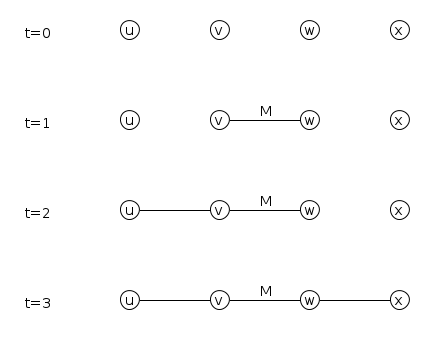
\includegraphics[width=0.5\textwidth]{example-4-3-1.png}
\caption{Illustration of example \ref{ex:naive-aug-path}}
\label{fig:example-4-3-1}
\end{figure}

\begin{example}
\label{ex:naive-aug-path}
Our dynamic graph $\mathcal{G}$ in this minimal example consists of $\mathcal{V}=\{u,v,w,x\}$ and the dynamic edge set $\mathcal{E}=( E_0 )$ with $E_0=\{\}$ on which we apply the sequence $S = ((1,v,w),(1,u,v),(1,w,x))$. Note that our matching in the beginning is empty, therefore $M_0=\{\}$. Using the naive approach applying $(1,v,w)$ to the graph, where the $1$ signs that we add the edge in this step, results in the matching $M_1=\{(v,w)\}$, since both vertices were free. If we now apply the next two sequence steps, the naive approach will not match any further edges, since for $(1,u,v)$ $v$ is already matched, and for $(1,w,x)$ $w$ is already matched. Therefore the matching after applying the last sequence step is $M_3=\{(v,w)\}$. It is easy to see, that we also have created an augmenting path of length $3$, starting at vertex $u$ and ending on $x$.
\end{example}

\noindent 
Neiman and Solomon address this issue by scanning the surroundings of any edge, that cannot be simply added to the matching for the reason that one endpoint of the edge is already matched. More specifically, if an edge $(u,v)$ cannot be added to the matching, because e.g. $u$ is already matched, we scan the neighbours of the mate of $u$, which we call $u'=\mate(u)$, for a free vertex $x$. By providing appropriate data structures this can be achieved in $O(\sqrt{n})$ time, which we will examine further in \todo{ref complexity}. If such a free vertex exists, we have found an augmenting path of length 3, which we invert. This increases the matching size by one. Further an edge insertion, where both endpoints are free, is processed as we already know, namely by simply adding this edge to the matching. Although detecting a vertex as free can be achieved in $O(1)$ time, matching an edge however entails updating several data structures, which takes $O(\sqrt{n+m})$ time as we will explain in a bit \todo{ref complexity}. An edge with both endpoints matched does not entail any further processing than the one needed to detect them as unfree. Reconsider the earlier example \ref{ex:naive-aug-path}, but this time using Neiman and Solomons approach to update the matching.

\begin{example}
\label{ex:ns-aug-path}
As before let the dynamic graph be $\mathcal{G}=(V,\mathcal{E})=(V,(E_0))=(\{u,v,w,x\},(\{\}))$ and the sequence $S=((1,v,w),(1,u,v),(1,w,x))$. We now apply $S$ on $\mathcal{G}$, where $i$ denotes the step and at each step we apply $S_i$.
\begin{enumerate}
	\item[i=0:] Since for the first step $M_0 = \{\}$ and therefore $v,w \notin M_0$ apply, the first edge $(v,w)$ is added directly to the matching. 	\item[i=1:] In the next step, we add $(u,v)$ to $\mathcal{G}$. Since $v$ is already matched, we check the surroundings of $\mate(v)$ for a free neighbour, however there exists none because the only neighbours of $v$ are $u$, which is $v$'s mate, and $w$, which is the other endpoint of the just added edge. 
	\item[i=2:] In the last step we add $(w,x)$. Again one endpoint is free, namely $x$, and the other one, $w$, is already matched. We scan the surroundings of $v=\mate(w)$ and detect $u$ as free neighbour of $v$. Therefore we have found an augmenting path starting at $x$ and ending at $u$. By inverting the augmenting path we receive the matching $M_3=\{(u,v),(w,x)\}$.
\end{enumerate}
Note that for this particular example the matching $M_3$ is a \emph{perfect} maximum matching. We call a matching \emph{perfect} if there is exists no free vertex.
\end{example}

\subsubsection{Edge Deletion}
\label{sec:ns-edge-out}

As mentioned in section \todo{ref to section naive approach, edge deletion} the process of edge deletion may create new augmenting paths of length $1$, which are simply edges with two free endpoints, but moreover may also create other augmenting paths of arbitrary length. In oder to tackle the augmenting paths of length $1$, the algorithm from Neiman and Solomon checks for both freed vertices whether they have free neighbours and if so matches the freed vertices with those free neighbours. This is done in $O(\sqrt{m})$ time. We examine this improvement in runtime over the naive approach with runtime $O(n)$ more thoroughly in section \todo{ref neiman,solomon - complexity}. 

We now focus on guaranteeing that no augmenting paths of length at most $3$ are present in the graph. First we will explain how augmenting paths of length $3$ can rise from an edge deletion using the following example.

\begin{example}
\label{ex:rise-aug-path}
Let $\mathcal{G}$ be a dynamic graph with $\mathcal{V}=\{u,v,w,x,y\}$ and $\mathcal{E}=\{E_0\}$, where $E_0=\{(u,v),(v,w),(w,x),(x,y)\}$ and let $M_0=\{(u,v),(w,x)\}$. Note that this graph and the respective matching can be easily obtained from applying the sequence $ R=((1,u,v),(1,w,x),(1,v,w),(1,x,y)) $ to an empty dynamic graph $\mathcal{G'}=(\mathcal{V},(\{\}))$. 

We now apply a single sequence step $S_0 = (0,u,v))$ to the dynamic graph~$\mathcal{G}$. Removing $(u,v)$ from the graph entails removing the edge also from the matching. This leaves the node $u$ free, but isolated, wherefore it can not be matched again. $v$ at the other hand is then starting point to an augmenting path of length 3, which ends at the free node $y$. Note that the matching $M_1=\{(v,w)\}$ is maximal, but only a 2-approximate to a maximum matching.
\end{example}

\noindent
Neiman and Solomon approach this by checking both freed vertices $u$ and $v$, if they are starting points to augmenting paths. This however does only happen, if the vertex degree is not more than a threshold of $\sqrt{2m}$, where $m$ denotes the amount of edges present in the graph at the moment of the update. For simplicity we will explain the further behaviour of the algorithm for the node $u$, the processing for $v$ is anyhow the same. Finding an augmenting path is done by scanning through all neighbours $w$ of $u$ and checking if $\mate(w)$ has a free neighbour. Naively this would take $O(\min(n,m))$ time, since the runtime complexity of checking all neighbours is dominated by the vertex degree. However as we mentioned previously, this approach is only taken for vertices with a degree less than $\sqrt{2m}$, time complexity is therefore reduced to $O(\sqrt{2m})$. The alternative behaviour will be explained subsequently. Now if an augmenting path has been found, we can invert it in $O(\log n)$ time (see \todo{ref}), hence the update time taken from this routine is $O(\sqrt{m})$.

For vertices with degree greater than $\sqrt{2m}$, we find a surrogate $z$ for $u$ with degree of at most $\sqrt{2m}$ who is the mate of a neighbour of $u$. We find such a surrogate by scanning linear through the neighbours of $u$, retrieving $z=\mate(w), w \in N(u)$, where $N(u)$ denotes the set of neighbours of $u$, and then checking if $\deg(z)\leq\sqrt{2m}$. Neiman and Solomon claim, that finding such a surrogate $z$ is done in at most $\sqrt{2m}$ steps, since otherwise the sum of degrees in the graph would be more than $\sqrt{2m} \cdot \sqrt{2m} = 2m$, which is impossible. Now that a surrogate vertex $z$ is found, we unmatch the edge $(w,z)$, match $(u,w)$ and handle $z$ then just as $u$ and $v$ were handled before. Since it is guaranteed, that $\deg{z}<\sqrt{2m}$, an infinite loop can be foreclosed.

We will give another example 

\begin{example}
\todo{todo}
\end{example}

\subsubsection{Approximation}
\label{sec:ns-approx}

As we tried to outline throughout the section, the goal of the algorithm is to maintain a maximal matching that is free from augmenting paths of length at most 3. Following \todo{cite hopcroft and karp} this approach guarantees, that the matching maintained is a $3/2$-approximate maximum matching.

\subsubsection{Complexity}
\label{sec:ns-complx}

In order to bound runtime complexity and guarantee deterministic behaviour, Neiman and Solomon use and maintain the following data structures. 

\begin{itemize}
\item The matching M is saved in an AVL-tree which suppports insertion and deletion in $O(\log n)$ time.
\item For each vertex $x \in \mathcal{V}$ an AVL-tree $N(x)$ is maintained, that holds all neighbours of $x$.
\item A custom data structure $F(x)$ for each vertex $x \in \mathcal{V}$, that contains all free neighbours of $x$ and supports insertion, deletion and querying, if a free neighbour exists, in $O(1)$ time and further allows retrieving a free node in $O(\sqrt{n})$ time.
\item Finally an addressable maximum heap $F_{max}$, which contains all free vetices indexed by their degree. This data structure supports insertion, deletion and updating keys in $O(\log n)$ time, as well retrieving the vertex with highest degree in $O(1)$ time.
\end{itemize}

\noindent
As mentioned earlier, detecting an augmenting path or detecting free vertices can be achieved in $O(\sqrt{n})$ or $O(1)$ time. However matching an edge is not as trivial as it might appear as it does entail updates on the data structure $F(w)$ for all $w \in N(x)$ for all $x \in \{u,v\}$. Naively this would mean update costs of $O(\deg(u) + \deg(v))$ time, which is $O(n)$, since the maximum degree for a vertex in a simple graph is $n-1$, where $n$. In order to bound this update time, Neiman and Solomon introduce two invariants, that state that:

\begin{invariant} 
All free vertices have degree at most $\sqrt{2n + 2m}$.
\end{invariant}

\begin{invariant} 
All vertices, that became free in round $i$ have degree at most $\sqrt{m}$.
\end{invariant}

\noindent
The handling of invariant 2 \todo{ref} has been already introduced, but implicitly. The action of finding a surrogate $z$ with $\deg(z)\leq\sqrt{2m}$ for a freed vertex $u$ with $\deg(u)>\sqrt{2m}$, where $u$ remains matched by matching the edge $(u,\mate(z))$, guarantees that any vertex freed in round $i$ has degree not more than $\sqrt{2m}$.

Invariant 1 \todo{ref} however has to be handled explicitly by identifying \emph{problematic} vertices, that are \emph{close} to violate \todo{ref inv 1}. They call a vertex \emph{problematic}, if it is free and its degree exceeds $\sqrt{2m}$. Neiman and Solomon prove, that it is sufficient to handle one vertex per sequence step additionally to the two vertices, which are already handled by being involved in the performed edge update. This one vertex is the vertex with maximal degree from all free vertices, which can be obtained from the maximum heap $F_{max}$ in $O(\log n)$ time (including removing this vertex from the heap as well as restoring the heap condition). This problematic vertex $x$ is then handled like a vertex $u$ of a freed edge $(u,v)$ with $\deg(u) > \sqrt{2m}$ is handled. This is, we find a surrogate $z$ for $x$, where $z=\mate(y)$, with $y \in N(x)$, unmatch $(z,y)$ in order to be able to match $(x,y)$ and let the surrogate vertex $z$ possibly become free. This however could create new augmenting paths of length $3$ which is why we then call the same procedure, which we use to find augmenting paths from a freed vertex after deletion of a matched edge, to assure that no such augmenting path exists.

\pagebreak
\section{Experimental Evaluation}
\label{sec:exp-eval}

In this section we present how we evaluated the implemented algorithms experimentally and what results we gathered. Our tests were performed on real-world graphs taken from the KONECT database. Since they provide only few dynamic graphs, we also present methods used to create dynamic sequences of edge insertions and deletions. We evaluate runtime and matching quality of the different algorithms in comparison to each other but also in comparison to the theoretically elaborated upper and lower bounds for runtime and matching quality respectively.

\subsection{Implementation and Environment}
\label{sec:impl-env}

In order to evaluate the previously presented algorithms experimentally, we implemented them in C++11 using g++ in version 5.5.0 as compiler. As a base for writing the code we used the KaHIP project. Unfortunately this project cannot be seen as an extension to KaHIP. The whole code is available at \todo{link to github repo} and is licensed under \todo{some license}.

Our experiments consisted of running different sequences, which will be further described in the following section \todo{section ref}. Every sequence was processed by every algorithm and data about time taken, graph edge cardinality, matching edge cardinality, average vertex degree and average vertex degree of matched vertices was gathered all $k$ steps, where $k$ is a custom parameter. In order to avoid corruption of data, especially the runtime, caused by external events on the test machine, every experiment was run several times and the runtime averaged.

As a benchmark we used GPA algorithm for maximal matching in static graphs to calculate the matchings for the static instances $G_i$ of the dynamic graph $\mathcal{G}$ at the points $i$ in time, where we also gathered the above mentioned data.

Further we also did comparison of all calculated matchings $M_i$, where$i$ is the same point in time $i$ already mentioned. More specifically for a given point in time $i$ we compared all matchings $M_i$ from all algorithms with each other by calculating the intersect of two matchings from two different algorithms. For $l$ algortihms this results in $\frac{l\cdot (l-1)}{2}$ calculated intersects. We did this to better examine the calculated matchings and gather insight to matching similarities.

As a test machine we used a system running Ubuntu 18.04.1 LTS on 4 cores, with 16GB RAM and 100GB disc space. Execution of experiments was done using \texttt{screen} sessions and also using \texttt{gnu parallel} in order to execute several sequential experiments in parallel. This however turned out to be a problem for very big input sequences (about 10M steps), causing memory issues and also consuming all disc space by saving the graph snapshots to files. Regarding the exhaustive use of RAM, we would like to mention, that we could not find any memory leaks using \texttt{valgrind} in our test programs.

\subsection{Input Graphs and Sequences}
\label{sec:inps-seqs}

\subsubsection{Creating Dynamic Sequences}
\label{sec:dyn-seqs}

We used several graphs from the \emph{Koblenz network collection} (\emph{KONECT}) as test data. Unfortunately only few of the provided graphs match our requirements of being dynamic, undirected, loop-free and without parallel edges. Since most of the graphs from KONECT are static, we used the following approaches to create dynamic graphs from the static ones provided. 

% Apart from converting KONECT graphs to sequences, that our test program can handle, we can also create sequences from a seed, where the endpoints for an edge, that is to be added are obtained randomly. The limitations in size for the output sequences which are given in the following do not apply to any sequences created from seed. A sequence created from seed is, at least theoretically, not limited in size.

\bigskip \noindent
\textbf{addition-only:} As the name already implies this approach does construct the static input graph by subsequently adding the edges of the static graph to the dynamic one in order of appearance. If the input graph provides time stamps as some of the KONECT graphs do, the edges are first sorted by time stamp and then added. The maximal size of such a sequence is therefore the size of the input sequence. Note that any unprocessed KONECT graph can be seen as a sequence.

\bigskip \noindent
\textbf{random-step:} Before a new sequence step is randomly set to either be an edge insertion or an edge deletion. If it is an edge insertion the next edge in order of appearance or if applicable sorted by time stamps is added to the sequence. Furthermore we maintain an array that contains all edges, that are present in the graph after the recently added sequence step. Hence if the next step is to be an edge deletion, an edge is randomly taken from the array of present edges added as edge deletion to the sequence. Further it gets deleted from the array of edges present in the graph. The maximal size of such a sequence is $2 \cdot l$, where $l$ is the length of the input sequence.

\bigskip \noindent
\textbf{sliding-window:} This approach takes an additional parameter $ws$ to determine the window size of the sliding window. For the first $ws$ sequence steps edges are added in order of appearance or sorted by time stamp. Note that we use $0$-based counting. Afterwards every edge $(u,v)$ added at step $k$ is removed again at step $i=ws+k$. For a input sequence of length $l$, that we convert into a sliding-window sequence, no edges are left to be inserted at step $2 \cdot l - ws$. After this point we continue by deconstructing the graph again by removing edges for the next $ws$ steps as before. The overall maximum length is then $2 \cdot l$ for a given input sequence of length $l$, further the window size $ws$ must not exceed the sequence length $l$.

\bigskip \noindent
\textbf{simple-outage:} As suggested from Bergamini and Meyerhenke we created sequences, where we remove a randomly chosen edge $(u,v)$ from the graph and then reinsert it in the next step. Similar to the sliding-window method, the first $ws$ sequence steps fill the graph up with edges. In the following phase we continue as already mentioned by removing and reinserting a randomly chosen edge. This method can be used to create arbitrary long sequences, however the window size $ws$ must not exceed the length of the input sequence $l$.

\bigskip \noindent
\textbf{pooled-outage:} As an extension to the simple-outage method this approach does not delete and then reinsert only one edge, but right after the insertion phase creates a pool of size $ps$ by removing $ps$ randomly selected edges. Afterwards we randomly decide for each step whether an edge from the pool is reinserted or another edge is deleted from the graph and therefore added to the pool. The edge cardinality is then expected to be approximately $ws-ps$, where $ws$ is the parameter determining the window size. Like the simple-outage method this approach can be used to create arbitrary long sequences, again the parameter $ws$ must not exceed the length of the input sequence $l$.

\subsubsection{Input Graphs}
\label{sec:in-graphs}

In table \ref{tab:graphs} we list all graphs that we either used to create dynamic sequences or that already were dynamic and could therefore be also processed natively.

\begin{table}
  \centering
    \begin{tabular}{| l | c | c | c | c |}
    	\hline
    	Name & $n = |G|$ & $m = |E|$ & Mode & Reference \\
    	\hline
%    	amazon & & & \\
%		dbpedia & & & \\
    	edit-enwiktionary & & & T & \\
    	edit-frwiktionary & & & T & \\
    	facebook-wosn-links & & & T & \\
    	flickr-growth & & & T & \\
    	link-dynamic-dewiki & & & D & \\
    	link-dynamic-frwiki & & & D & \\
    	link-dynamic-itwiki & & & D & \\
    	link-dynamic-nlwiki & & & D & \\
    	link-dynamic-plwiki & & & D & \\
    	link-dynamic-simplewiki & & & D & \\
    	livejournal-groupmemberships & & & S & \\
    	orkut-groupmemberships & & & S & \\
    	\hline
    \end{tabular}
  \caption{Input graphs from KONECT. S stands for a static graph instance, T for graphs with time stamps and D for dynamic graphs}
  \label{tab:graphs}
\end{table}

We created from each of the graphs in table \ref{tab:graphs} the 10 sequences seen in \ref{tab:seq-params}. Additionally we ran all real dynamic graphs also as the native sequence they represent. As we mentioned before, we ran into troubles with RAM when processing very large sequences. Hence we truncated the input sequences in length and also in number of vertices, since otherwise it could happen that the graph would become extremly sparse. 

\begin{table}
  \centering
    \begin{tabular}{| l | c | c | c | c |}
    	\hline
    	Method & $l$ & $n_{max}$ & $ws$ & $ps$ \\
    	\hline
		addition-only & 1000000 & 100000 & - & - \\
		pooled-outage & 1000000 & 100000 & 100000 & 10\% \\
		pooled-outage & 1000000 & 100000 & 500000 & 10\% \\
		pooled-outage & 2000000 & 100000 & 1000000 & 10\% \\
		pooled-outage & 3000000 & 100000 & 1500000 & 10\% \\
		pooled-outage & 4000000 & 100000 & 2000000 & 10\% \\
		pooled-outage & 5000000 & 100000 & 2500000 & 10\% \\
		random-step & 1000000 & 100000 & - & - \\
		simple-outage & 1000000 & 100000 & 100000 & - \\
		sliding-window & 1000000 & 100000 & 100000 & - \\
    	\hline
    \end{tabular}
  	\caption{Parameters used for creating sequences. $l$ denotes the sequence length, $n_{max}$ the maximal vertex ID. $ws$ and $ps$ are window size and pool size as percentage of the window size respectively as introduced in \ref{sec:}.}
    \label{tab:seq-params}
\end{table}


\subsection{Results}
\label{sec:results}
\todo{todo}

\pagebreak
\section{Conclusion}
\label{sec:conclusion}

\pagebreak

\bibliographystyle{acm}
\bibliography{BSc_Latex_Template}

\end{document}
% End of document.